% ============================================================
%  Extended abstract (4 pages) -- BTP final report
%  Compile with pdfLaTeX. Figures in ./figures
% ============================================================
\documentclass[11pt,a4paper]{article}
\usepackage[T1]{fontenc}
\usepackage[utf8]{inputenc}
\IfFileExists{newtxtext.sty}{\usepackage{newtxtext,newtxmath}}{\usepackage{mathptmx}}
\usepackage[a4paper,margin=20mm]{geometry}
\usepackage{graphicx,booktabs,amsmath,tabularx,float}
\usepackage[labelsep=colon,font=small,skip=3pt]{caption}
\usepackage{titlesec}
\usepackage[hidelinks]{hyperref}
\graphicspath{{figures/}}
\setlength{\parindent}{0pt}
\setlength{\parskip}{5pt}
\setlength{\emergencystretch}{1.5em}
\setlength{\textfloatsep}{8pt plus 2pt}
\setlength{\floatsep}{6pt plus 2pt}
\setlength{\intextsep}{6pt plus 2pt}
\titleformat{\section}{\bfseries\large}{\thesection}{0.6em}{}
\titlespacing*{\section}{0pt}{8pt}{2pt}
\titleformat{\subsection}{\bfseries}{\thesubsection}{0.6em}{}
\titlespacing*{\subsection}{0pt}{5pt}{1pt}
\pagestyle{plain}

\newcommand{\Uinf}{U_\infty}
\newcommand{\Cd}{C_d}
\newcommand{\Cf}{C_f}
\newcommand{\dn}{\delta_{99}}

\begin{document}

\begin{center}
{\Large\bfseries Turbulent Flow behind a Flat Plate Mounted Normal to the Wall}\\[4pt]
{\large Extended Abstract}\\[6pt]
\textbf{Ankit Kumar Modi \& Gaurav Waghmare}\\[2pt]
Supervisor: Prof.\ Arjun Sharma\\[2pt]
Department of Applied Mechanics, Indian Institute of Technology Delhi --- November 2026
\end{center}
\vspace{-2pt}
\hrule
\vspace{4pt}

{\small
\textbf{Summary.} The turbulent flow in the corner of an L-shaped wall--plate junction (460\,mm long, $Re_L = 1.13\times10^{6}$) is computed with steady RANS (ANSYS Fluent, SST $k$--$\omega$, $y^+<1$) on three grids (0.53--2.53 M cells). The fine-grid drag coefficient is $\Cd = 0.0617$ (GCI 4.6\%). The blunt leading edge produces the strongest stagnation at the inside corner and a separation bubble that is shorter near the junction. A counter-rotating corner vortex pair with unequal strengths redistributes momentum: low-momentum fluid moves into the corner along the walls and out along the bisector, while high-momentum fluid is brought towards the walls 15--30\,mm from the corner. Corner skin friction is 30--50\% lower than away from the junction and up to 32\% higher in the downwash band. The corner circulation decays by about 9.5 times along the plate.
\par}
\vspace{2pt}
\hrule

\section{Introduction and objectives}
Where a body meets a wall---a wing on a fuselage, a fin on a hull---the two boundary layers meet in a corner. This \emph{junction flow} contains leading-edge vortices, cross-stream (secondary) motion along the corner and local changes of wall shear (Simpson, 2001). The project is based on the experiment of Nakayama and Rahai (1984), who measured mean and secondary velocities, Reynolds stresses and skin friction behind a flat plate mounted normal to a wall.

Secondary flows are of two kinds (Bradshaw, 1987). Flows of \emph{Prandtl's first kind} arise when existing vorticity is tilted by the mean flow, as in the horseshoe vortex of a wing--body junction. Flows of the \emph{second kind} are driven by Reynolds-stress anisotropy in a straight corner (Gessner, 1973) and are weak, about 1--3\% of the main velocity. Vorticity is solenoidal, $\nabla\cdot\boldsymbol{\omega}=0$, so vortex lines cannot end in the fluid. The SST model (Menter, 1994) cannot represent the second-kind mechanism (Pope, 2000).

The mid-semester model (a T-shape in a small box with no-slip side walls, 10\,mm tetrahedra and no inflation) was qualitative: duct blockage accelerated the flow to 41.8\,m/s instead of 36\,m/s. The objectives of the final phase were: (i) a corrected, verified simulation with a three-grid study (Celik et al., 2008); (ii) a physical interpretation of how the floor and plate boundary layers interact at the junction; and (iii) a quantitative comparison of the corner with regions far from it.

\section{Formulation and methodology}
The L consists of a vertical plate and a floor plate, each $460\times320\times10$\,mm with square edges, inside a $2.0\times0.60\times0.50$\,m box (Fig.~\ref{fig:geom}). The inside corner runs along $x=y=0.01$\,m, the leading and trailing edges (LE, TE) are at $z=\pm0.23$\,m and the flow is in $-z$. Air ($\rho=1.225$\,kg/m$^3$, $\mu=1.7894\times10^{-5}$\,kg/(m\,s)) enters at $\Uinf=36$\,m/s ($I=1\%$, $\mu_t/\mu=10$); the outlet is at 0\,Pa and the four lateral faces are symmetry planes. The coupled pseudo-transient solver with second-order schemes is used.

\begin{figure}[H]
\centering
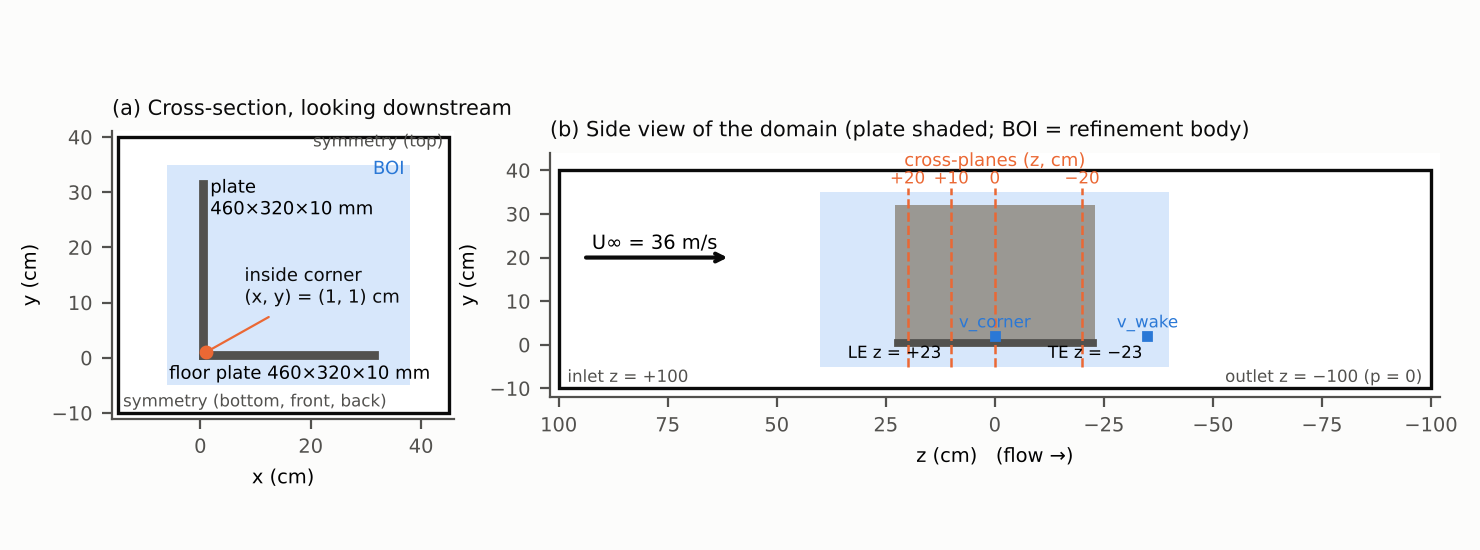
\includegraphics[width=0.66\textwidth]{fig2_1.png}\hfill
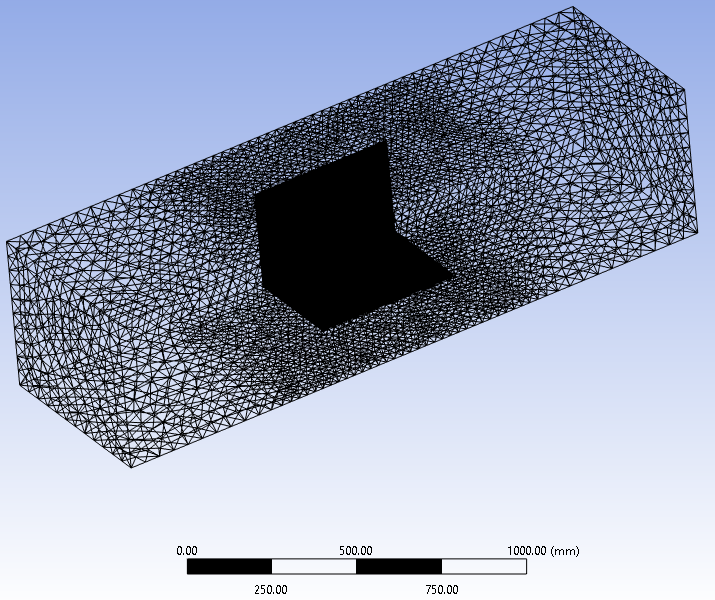
\includegraphics[width=0.32\textwidth]{fig2_2.png}
\caption{Left: geometry, domain, refinement body (BOI), cross-planes and monitor points. Right: fine mesh of the L inside the enclosure (2.53 M cells).}
\label{fig:geom}
\end{figure}

The mesh uses tetrahedra with 25 prism layers on all L faces (first layer 0.01\,mm, growth 1.2, total $\approx4.7$\,mm). Only the face and BOI sizes were changed between grids, giving an effective refinement ratio of about 1.30. The fine mesh has maximum skewness 0.80; about 0.1\% of cells, at the outer free edge of the floor away from the junction, have low orthogonal quality. Drag on all L faces gives $\Cd = F_D/(\tfrac12\rho\Uinf^2A_\mathrm{ref})$ with $A_\mathrm{ref}=0.1472$\,m$^2$. Velocity monitors are placed in the corner at $(0.02,0.02,0)$\,m and in the corner wake at $(0.02,0.02,-0.35)$\,m. Cross-planes at $z=+0.20$, $+0.10$, 0 and $-0.20$\,m ($s=30$, 130, 230 and 430\,mm from the LE) are sampled over $60\times60$\,mm from the inner walls. Positive and negative streamwise vorticity are integrated separately as $\Gamma^+$ and $\Gamma^-$. Skin friction is compared in a corner band (0--4\,mm), a downwash band (15--30\,mm) and a reference band (60--150\,mm).

\section{Results and discussion}
\subsection{Verification}
Over the final 200 iterations the drag varies by $\le0.05\%$ and the velocity monitors by $\le0.9\%$. The mass imbalance is below $2\times10^{-4}\%$ and the maximum $y^+$ is 0.77--0.93. Table~\ref{tab:grid} and Fig.~\ref{fig:grid} summarise the grid study. Drag changes by 1.43\% from the medium to the fine grid (GCI 4.6\%). For the corner speed the apparent order (4.2) exceeds the formal second order, so the 2.7\% GCI is a lower bound; limiting the order to 2 gives about 8\%. The wake differences grow, so no reliable GCI exists for the wake. The fine grid is used for all further results.

\begin{table}[H]
\centering\small
\begin{tabular}{@{}lllllll@{}}
\toprule
Grid & $N$ (M) & $h$ (mm) & $\Cd$ & $U_\mathrm{corner}$ (m/s) & $U_\mathrm{wake}$ (m/s) \\
\midrule
Coarse & 0.529 & 10.41 & 0.063731 & 33.195 & 28.569 \\
Medium & 1.150 & 8.04  & 0.062529 & 29.546 & 27.162 \\
Fine   & 2.528 & 6.18  & 0.061649 & 28.304 & 25.600 \\
\midrule
Extrapolated / GCI & -- & -- & 0.0594 / 4.6\% & 27.69 / 2.7\% ($\approx$8\% with $p=2$) & not defined \\
\bottomrule
\end{tabular}
\caption{Three-grid study (final-200-iteration means).}
\label{tab:grid}
\end{table}

\begin{figure}[H]
\centering
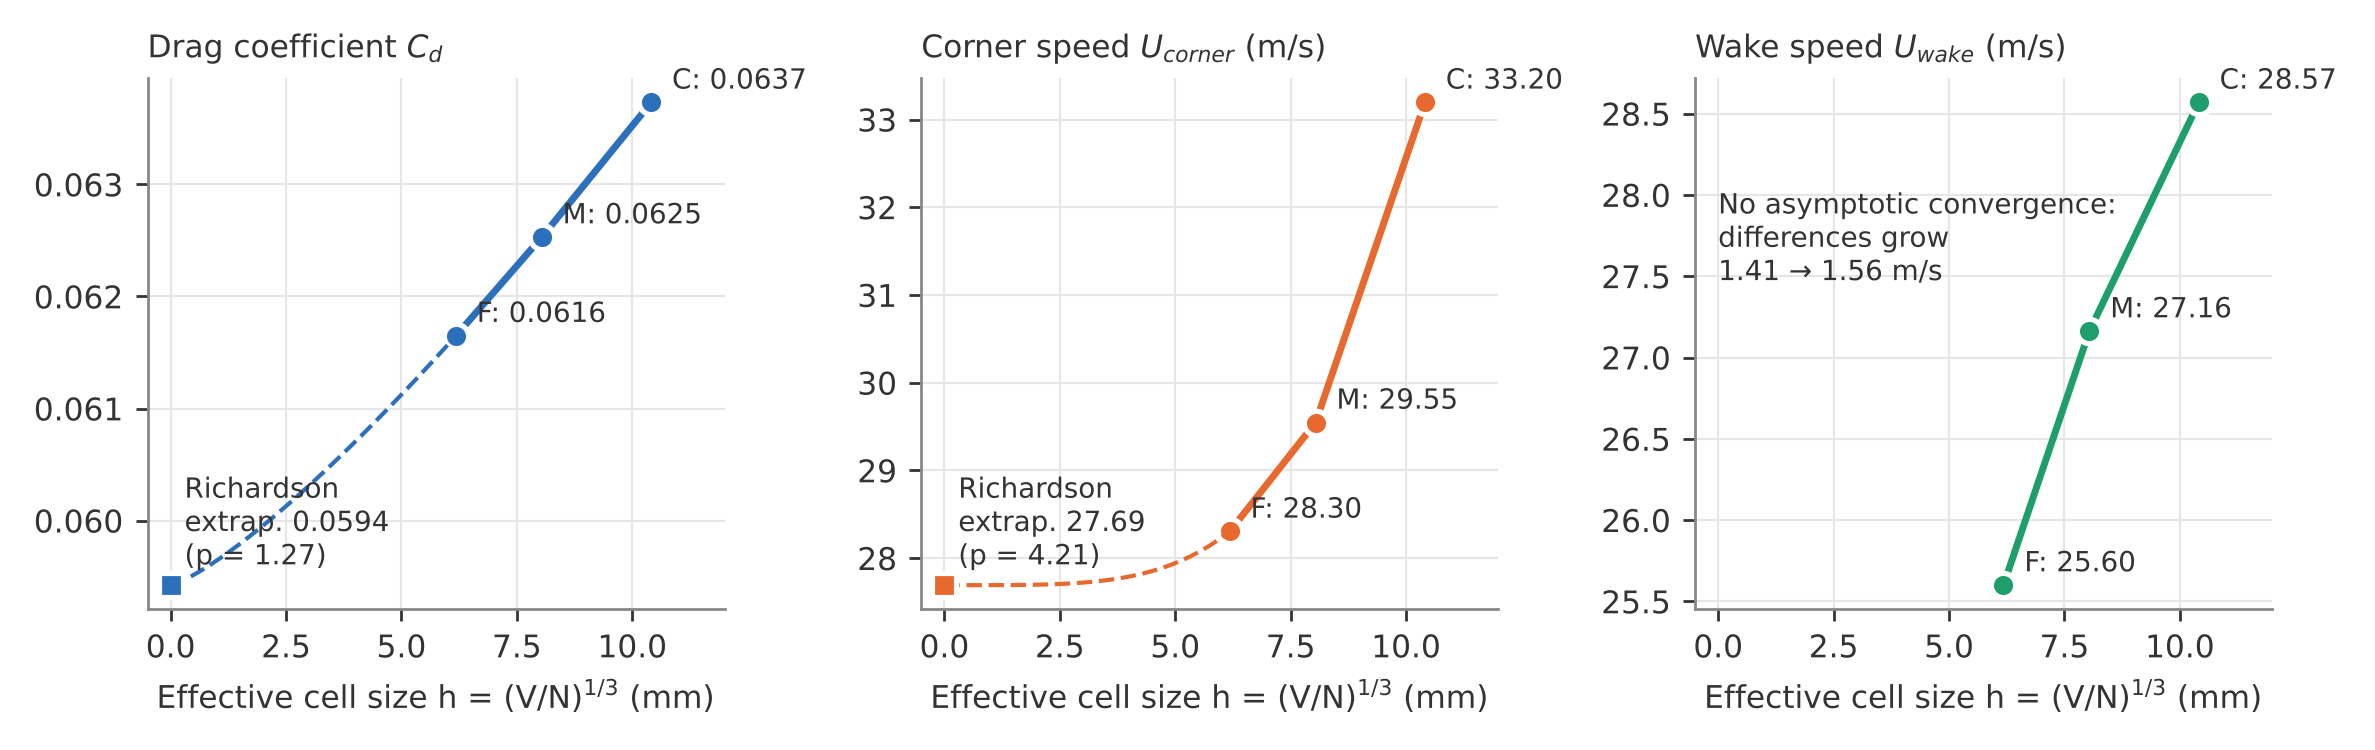
\includegraphics[width=0.7\textwidth]{fig3_2.png}
\caption{Grid convergence of $\Cd$, corner speed and wake speed versus effective cell size $h=(V/N)^{1/3}$, with Richardson extrapolation.}
\label{fig:grid}
\end{figure}

\subsection{Leading edge and boundary layers}
The largest stagnation region lies at the inside corner of the blunt front face, where both plates obstruct the oncoming flow. The 2\% overshoot of the peak pressure (837\,Pa) above the inlet total pressure (819\,Pa) is a local discretisation error at the sharp edge. Flow separates at the square edges. On the floor the reversed shear extends 70--77\,mm far from the plate but only 40--50\,mm within 30\,mm of it, so the junction shortens the separation bubble.

At mid-length, far from the junction, the floor and plate layers are alike: $\dn = 25.6$/26.0\,mm, $\delta^*=6.12$/6.34\,mm and $H=1.66$/1.64. These are about four times thicker than the flat-plate estimate (6\,mm), a consequence of recovery after the LE separation. Near the corner the profiles are fuller (28.4\,m/s at $d=10$\,mm versus 26.0--26.7\,m/s far away). Along the bisector, 99\% of $U_e$ is reached 27.3\,mm from the corner, only 19\,mm from each wall, which is less than $\dn$. The corner region therefore carries more momentum than either boundary layer alone (Fig.~\ref{fig:profiles}).

\begin{figure}[H]
\centering
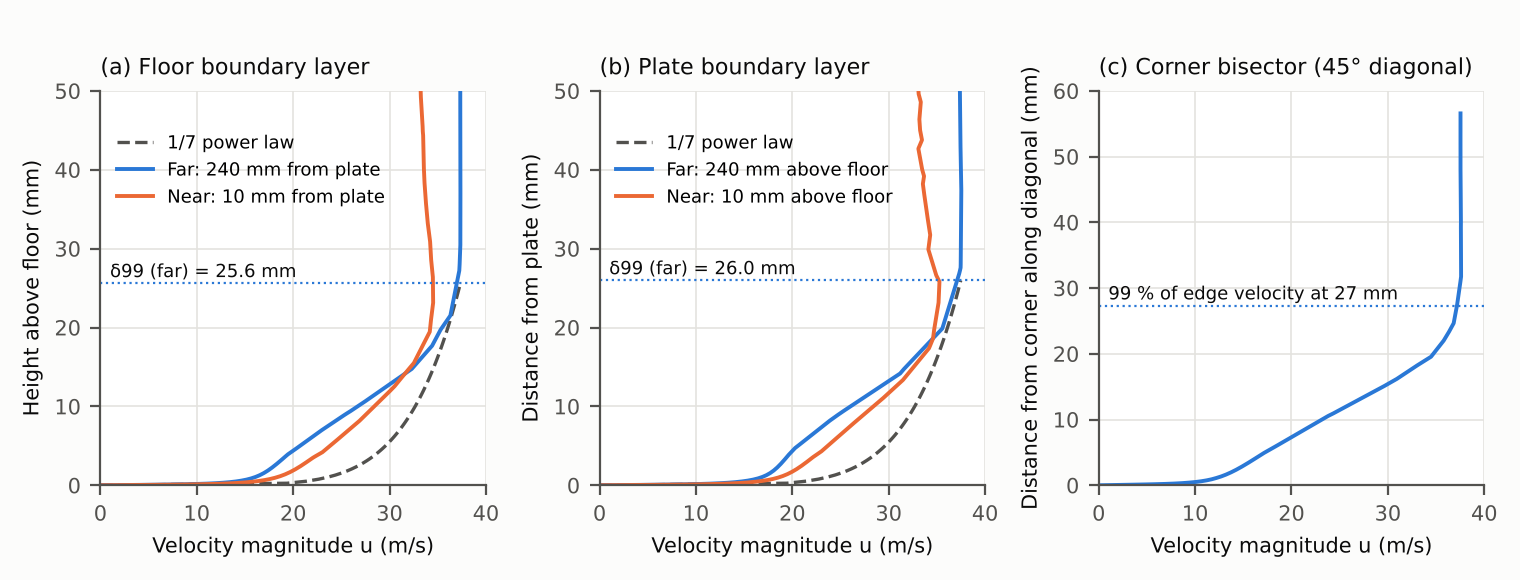
\includegraphics[width=0.62\textwidth]{fig3_3.png}
\caption{Velocity-magnitude profiles at mid-length, far from (240\,mm) and near (10\,mm) the other wall, and along the corner bisector.}
\label{fig:profiles}
\end{figure}

\subsection{Corner vorticity}
The floor layer carries $\omega_x<0$ and the plate layer $\omega_y>0$ (wall values of order $10^5$\,s$^{-1}$). Near the corner these layers interact, and streamwise vorticity $\omega_z$ appears (Fig.~\ref{fig:wz}). Its transport equation,
\begin{equation}
(\mathbf{u}\cdot\nabla)\,\omega_z = \omega_x\frac{\partial w}{\partial x} + \omega_y\frac{\partial w}{\partial y} + \omega_z\frac{\partial w}{\partial z} + \nu\nabla^2\omega_z - \big[\nabla\times(\nabla\cdot\mathbf{R})\big]_z ,
\end{equation}
shows that the wall vorticity can be tilted into the streamwise direction by the spanwise gradients of $w$ (first two terms), which are largest at the blunt LE. Downstream of the bubble, positive $\omega_z$ lies beside the plate and negative $\omega_z$ above the floor, centred 5--20\,mm from the walls. This forms a counter-rotating corner pair.

\begin{figure}[H]
\centering
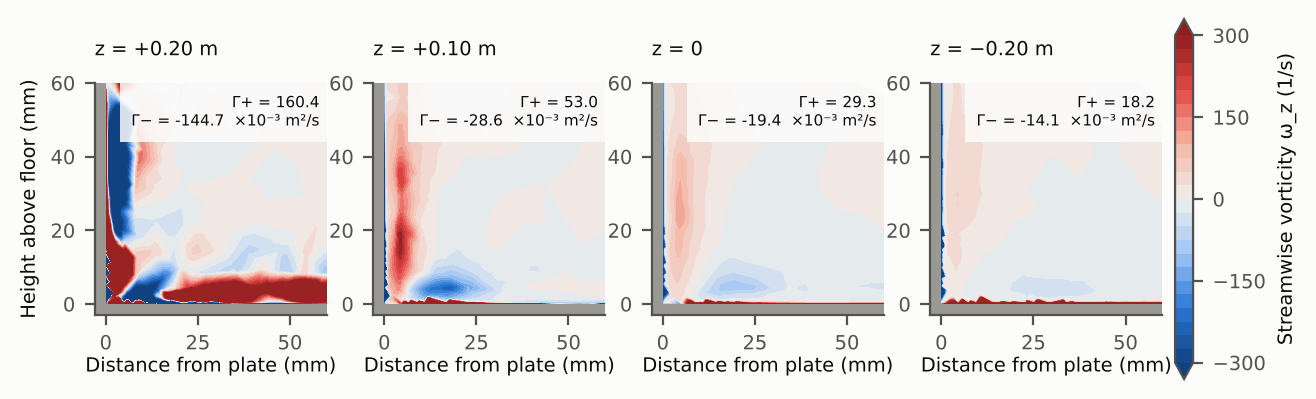
\includegraphics[width=0.84\textwidth]{fig3_5.png}
\caption{Streamwise vorticity on the four cross-planes ($s=30$, 130, 230 and 430\,mm); colour limits $\pm300$\,s$^{-1}$.}
\label{fig:wz}
\end{figure}

The two cells are unequal (Fig.~\ref{fig:circ}): the plate-side cell is 1.11--1.85 times stronger at every station. The total circulation $\Gamma^++|\Gamma^-|$ falls from 305.1 to $32.3\times10^{-3}$\,m$^2$/s, a factor of 9.5 between $s=30$ and 430\,mm. A factor of 3.7 of this occurs before $s=130$\,mm, where the LE bubble reattaches. This supports a leading-edge (first-kind) origin of the corner vortices, although a full vorticity budget was not computed.

\begin{figure}[H]
\centering
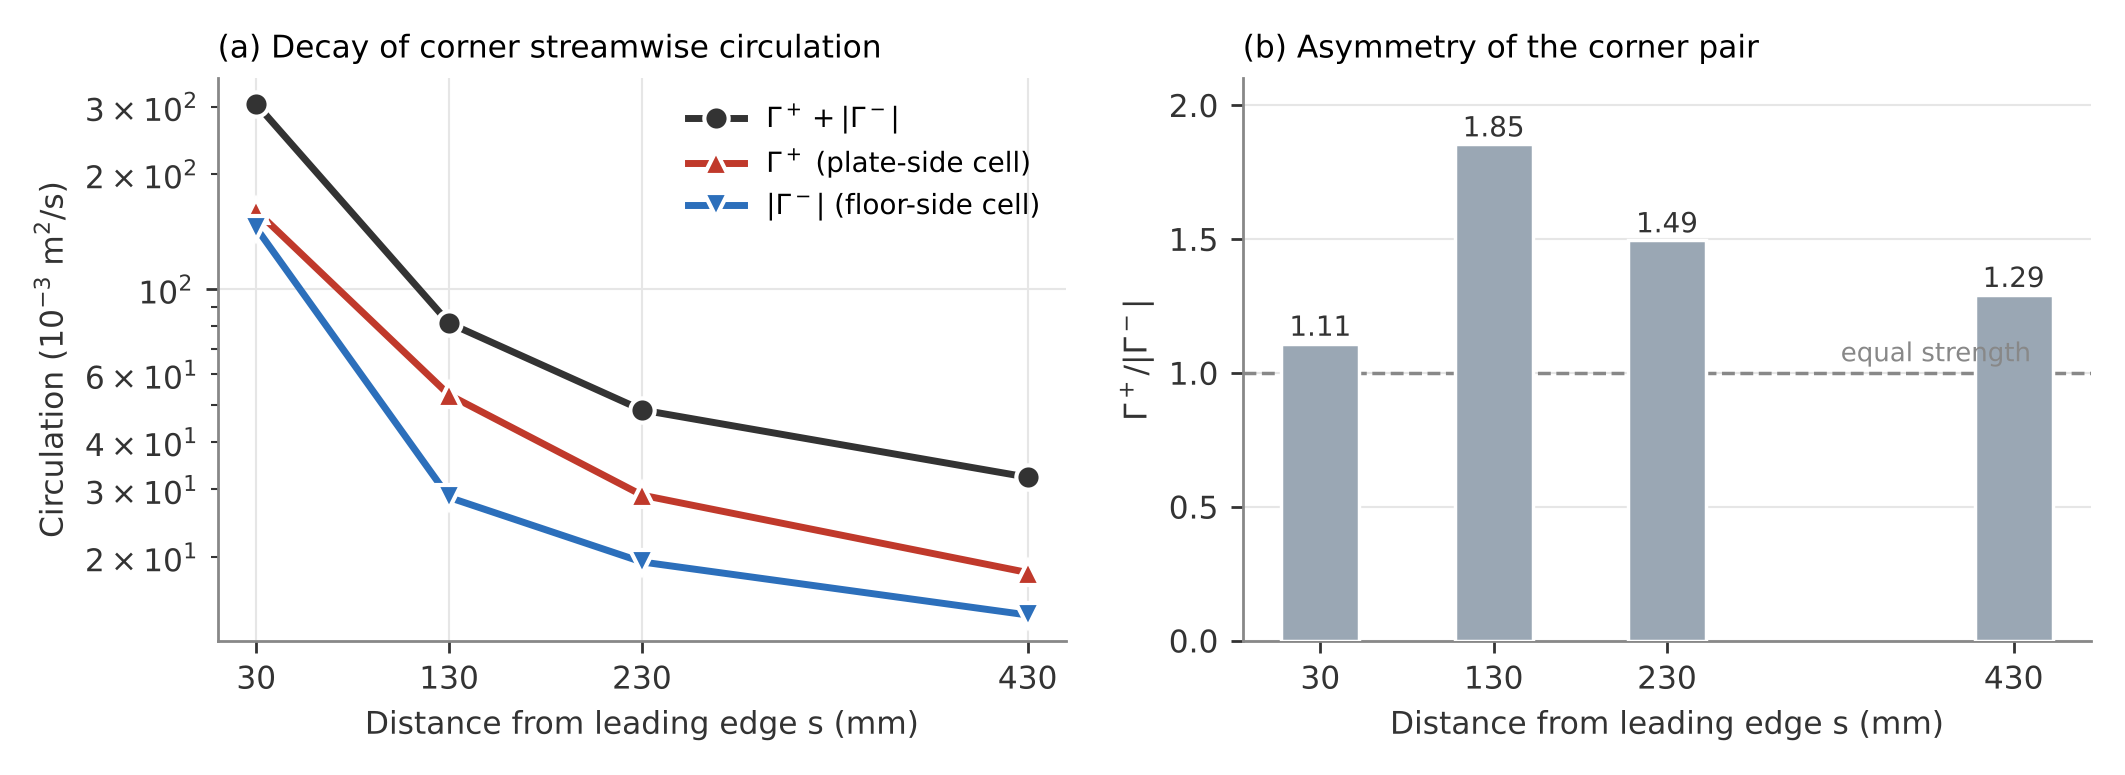
\includegraphics[width=0.58\textwidth]{fig3_6.png}
\caption{(a) Decay of corner circulation with distance from the LE; (b) asymmetry ratio $\Gamma^+/|\Gamma^-|$.}
\label{fig:circ}
\end{figure}

\subsection{Secondary flow and wall shear}
At $s=130$ and 230\,mm, the cross-flow within about 3\,mm of each wall points into the corner (0.1--0.46\,m/s) and leaves along the bisector (0.07--0.28\,m/s), as shown in Fig.~\ref{fig:iso}. On the outer side of each cell, high-momentum fluid is brought towards the walls 15--30\,mm from the corner, so the isovels bend towards the walls. Near the LE the cross-flow reaches 3.5\,m/s (10\% of $\Uinf$) and is dominated by displacement from the blunt edge; downstream it is about 1\% of $\Uinf$.

\begin{figure}[H]
\centering
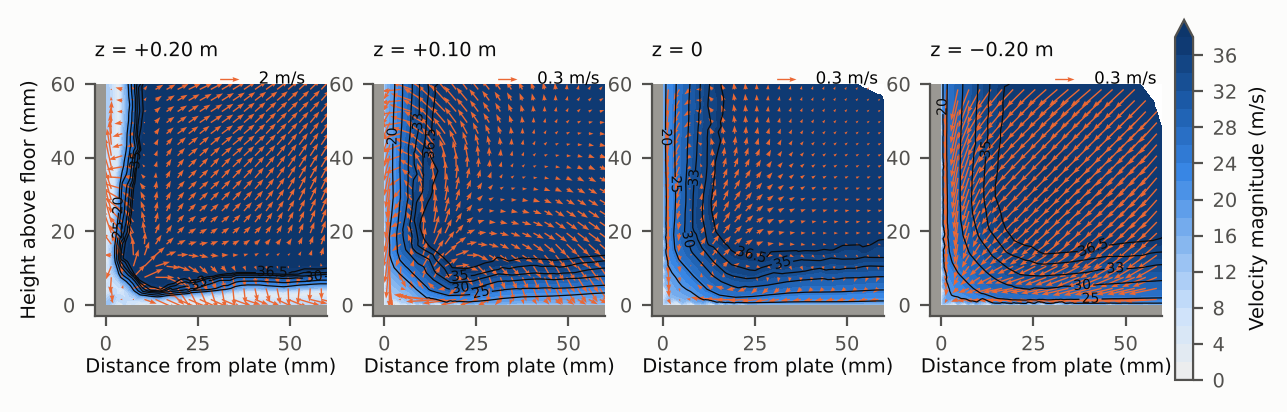
\includegraphics[width=0.84\textwidth]{fig3_7.png}
\caption{Isovels (black, m/s) and cross-flow vectors on the four planes (reference arrow 2\,m/s in the first panel, 0.3\,m/s in the others).}
\label{fig:iso}
\end{figure}

The secondary flow leaves a clear imprint on the skin friction (Fig.~\ref{fig:cf}). Within 4\,mm of the corner, $\Cf$ is 30--50\% below the reference band (e.g.\ $1.05\times10^{-3}$ versus $2.16\times10^{-3}$ on the floor at $s=130$\,mm). This is partly geometric, because the shear vanishes into a $90^\circ$ corner. In the 15--30\,mm downwash band, the floor $\Cf$ is 32\% above the reference value at $s=130$\,mm, falling to 12\% and 8\% downstream. The plate enhancement is smaller (13\%, 0\% and 2\%), consistent with the unequal cell strengths.

\begin{figure}[H]
\centering
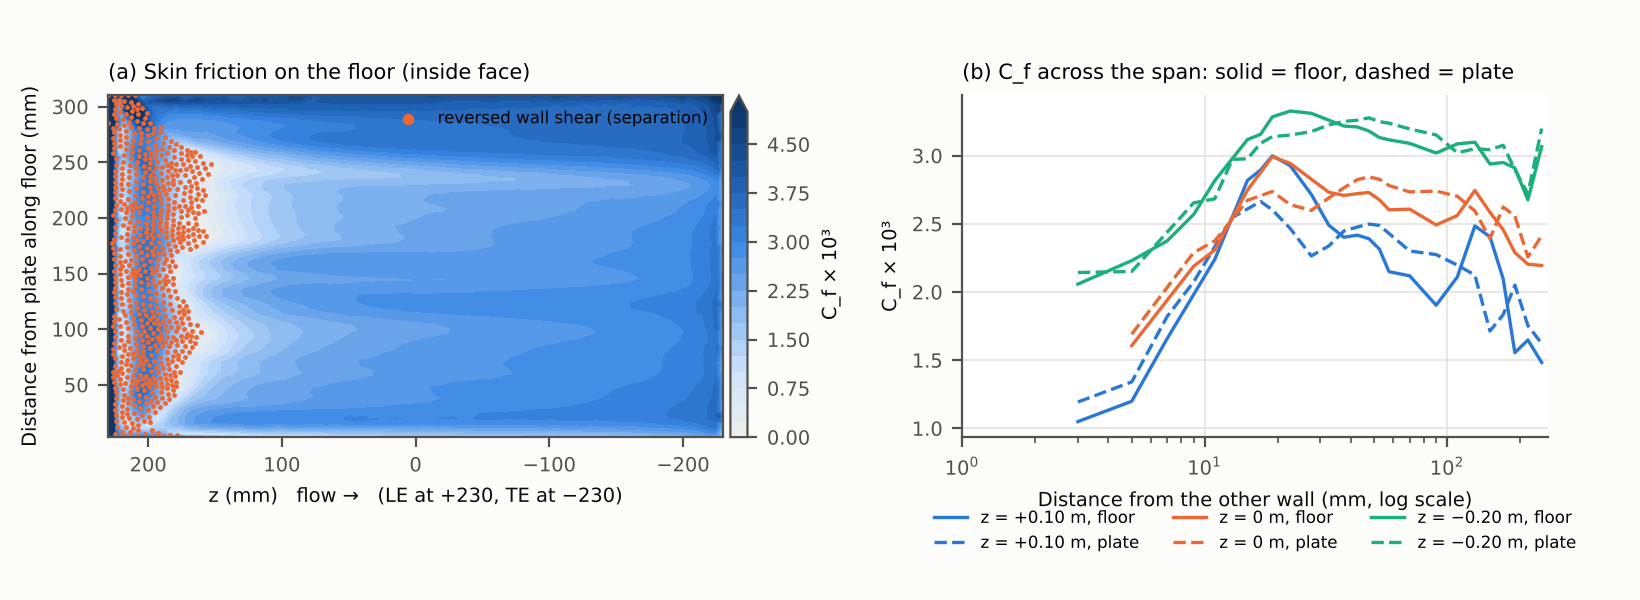
\includegraphics[width=0.68\textwidth]{fig3_8.png}
\caption{(a) Floor skin friction with the reversed-shear region marked; (b) $\Cf$ versus distance from the other wall (solid: floor, dashed: plate).}
\label{fig:cf}
\end{figure}

\section{Conclusions}
\begin{enumerate}\setlength{\itemsep}{1pt}
\item The corrected RANS model has $y^+<1$, mass balance and bounded monitors. The fine-grid $\Cd=0.06165$ (GCI 4.6\%) and the corner speed (GCI 2.7--8\%) are grid-converged; the corner-wake speed is not.
\item The blunt LE creates the strongest stagnation at the inside corner and a separation bubble that is shorter near the junction (40--50\,mm) than far from it (70--77\,mm).
\item A counter-rotating corner vortex pair, with the plate-side cell 1.1--1.9 times stronger, decays about 9.5 times along the plate, mostly within the first 130\,mm. This is consistent with tilting of wall vorticity at the leading edge.
\item The secondary flow makes the corner region fuller than either boundary layer. It lowers $\Cf$ by 30--50\% in the corner and raises it by up to 32\% in the downwash band.
\end{enumerate}
\textbf{Limitations and future work.} SST cannot capture second-kind (stress-driven) secondary flow, and the comparison with Nakayama and Rahai (1984) is qualitative because their incoming boundary layer was fully developed. Future work includes a Reynolds-stress or corner-corrected model, a longer domain with a refined corner wake, vortex-line analysis and the NACA 0010 wing--body junction.

{\footnotesize
\section*{References}
\setlength{\parskip}{0pt}
Bradshaw, P. (1987). Turbulent secondary flows. \emph{Annu.\ Rev.\ Fluid Mech.}\ 19:53--74. \quad
Celik, I.\,B. et al.\ (2008). Procedure for estimation and reporting of uncertainty due to discretization in CFD applications. \emph{J.\ Fluids Eng.}\ 130:078001. \quad
Gessner, F.\,B. (1973). The origin of secondary flow in turbulent flow along a corner. \emph{J.\ Fluid Mech.}\ 58:1--25. \quad
Menter, F.\,R. (1994). Two-equation eddy-viscosity turbulence models for engineering applications. \emph{AIAA J.}\ 32:1598--1605. \quad
Nakayama, A. and Rahai, H.\,R. (1984). Measurements of turbulent flow behind a flat plate mounted normal to the wall. \emph{AIAA J.}\ 22:1817--1819. \quad
Pope, S.\,B. (2000). \emph{Turbulent Flows.} Cambridge University Press. \quad
Simpson, R.\,L. (2001). Junction flows. \emph{Annu.\ Rev.\ Fluid Mech.}\ 33:415--443.
\par}

\end{document}
